% Materials and Methods
%This chapter elaborates on all working steps that were necessary to build, test, and evaluate the system, and all of its components. First, the methodology we used to solve the research question is explained. Then, all hardware components and software programs, that were used during the development process, are listed. Afterwards, the data pipeline (i.e. data collection, data pre-processing algorithms, and feature extraction), the experiment setup we used to build the database, and finally machine learning algorithms and evaluation methods.
In this chapter, we present all the hardware components and software applications that were used in the process of this thesis.

\section{Hardware}
%All experiments and measurements were conducted within the facilities of Systems Neuroscience and Neurotechnology Unit, particularly the Green Lab, located at the University Hospital Saarland, and the Mindscan Lab, located at the HTW Saar (Technikum).

\subsection{Empatica E4}\label{e4spec}
The Empatica E4 wristband is a wearable wireless device designed for comfortable, continuous, real-time data acquisition. It is a class IIa medical device in the EU, according to CE Cert. No. 1876/MDD (93/42/EEC Directive) and was designed for daily life usage \cite{e4}.

\begin{figure}[ht]
	\centering
  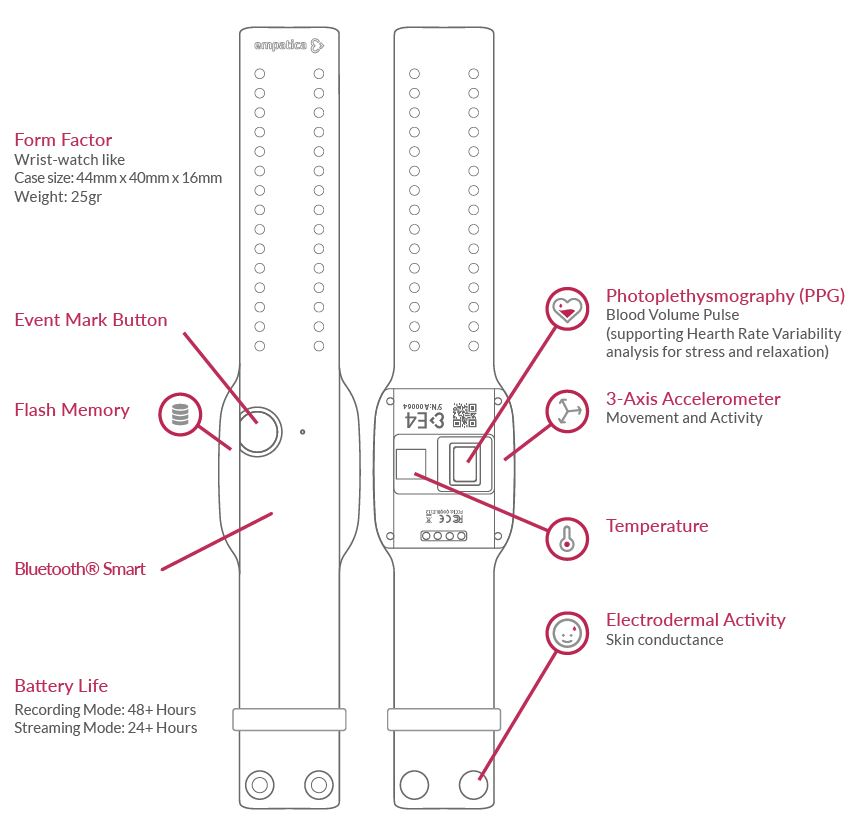
\includegraphics[width=0.7\textwidth]{images/E4overview.JPG}
	\caption{Overview of the Empatica E4 wristband.}
	\label{e4overview}
\end{figure}

Figure \ref{e4overview} shows an overview of the entire E4 wristband from either side indicating key attributes as wells as a total of four different sensors that will be discussed briefly in the following:

\begin{itemize}
\item \textbf{Photoplethysmography (\gls{ppg})} to provide blood volume pulse (\gls{bvp}), from which heart rate, heart rate variability and other cardiovascular features may be derived
\item \textbf{Electrodermal activity (\gls{gsr})} is used to measure sympathetic nervous system arousal and to derive features related to stress, engagement and excitement
\item \textbf{3-Axis accelerometer} to capture motion-based activity
\item \textbf{Infrared thermopile} for reading skin temperature
\end{itemize}

As the E4 is intended to be worn on the wrist these sensors are set up in a specific way to provide for optimal use. As can be seen on \ref{e4overview} the majority of the sensors are located on the backside of the main unit not including the \gls{gsr}-sensor, which is located on the wristband itself.\\
Wearing the E4 wristband is equally intrusive to wearing a watch and therefore providing a high level of convenience compared to other physiologic measures such as electrocardiogram \gls{ecg} or electroencephalogram \gls{eeg}.\\

\subsubsection{Sampling Specifications}
All recordings were performed using only software licensed by Empatica. Using the approved streaming server application and the compatible Bluetooth dongle, the recorded data was streamed directly to an operator's personal computer via a Bluetooth connection. 

\subsubsection{EDA sensor}
\begin{itemize}
\item Sampling frequency: 4 Hz (Non customizable).
\item Resolution: 1 digit ~900 pSiemens.
\item Range: 0.01 $\mu$Siemens – 100 $\mu$Siemens.
\item Alternating current (8Hz frequency) with a
max peak to peak value of 100 $\mu$Amps (at 100
$\mu$Siemens).
\item Electrode(Placement): on the ventral (inner) wrist.
\item Electrode(Build): Snap-on, silver (Ag) plated with metallic core.
\item Electrode(Longevity): 4–6 months
\end{itemize}

\subsubsection{PPG sensor}
\begin{itemize}
\item Sampling frequency 64 Hz (Non customizable).
\item LEDs: Green (2 LEDs), Red (2 LEDs) Photodiodes: 2
units, total 15.5 $mm^{2}$ sensitive area.
\item Sensor output: Blood Volume Pulse (BVP) (variation
of volume of arterial blood under the skin resulting
from the heart cycle).
\item Sensor output resolution 0.9 nW / Digit.
\item Motion artifact removal algorithm: Combines different light wavelengths. Tolerates external lighting conditions.
\end{itemize}

\subsubsection{Infrared Thermopile}
\begin{itemize}
\item Sampling frequency: 4 Hz (Non customizable).
\item Range(Ambient temperature): -40...85$\deg$C (if available).
\item Range(Skin temperature): -40...115$\deg$C.
\item Resolution: 0.02$\deg$C.
\item Accuracy $\pm$0.2$\deg$C within 36-39$\deg$C.
\end{itemize}

\subsubsection{Real-time clock}
\begin{itemize}
\item Resolution(Recording mode): 5s synchronization resolution. Average of 6 seconds in 6 million seconds drift.
\item Resolution(Streaming mode): Temporal resolution up to 0.2 seconds with connected device.
\end{itemize}

\subsection{Processing Unit}
The processing unit it the expression given to the computer, which is used to run any software that is essential for data transmission and data processing, such as the Empatica streaming server application, MATLAB, and PyCharm. We used a Lenovo ThinkPad, with an Intel(R) Core(TM) i5-6200U, CPU @ 2.3 GHz, 8 GB RAM, running a 64-Bit version of Windows 10. 

\section{Software}
\subsection{E4 Streaming Server}
The E4 streaming server for Windows (version of May,2018) is a software application that allows to forward real-time data of one or multiple Empatica E4 devices to one or multiple TCP socket connections. However, as each TCP connection is limited to receiving data from only one Empatica E4 device, the connection to multiple devices would also require multiple TCP connections. The E4 streaming server is intended to provide access to the data streams using scripts and applications of any programming language \cite{E4SS}.\\

\begin{figure}[ht]
	\centering
  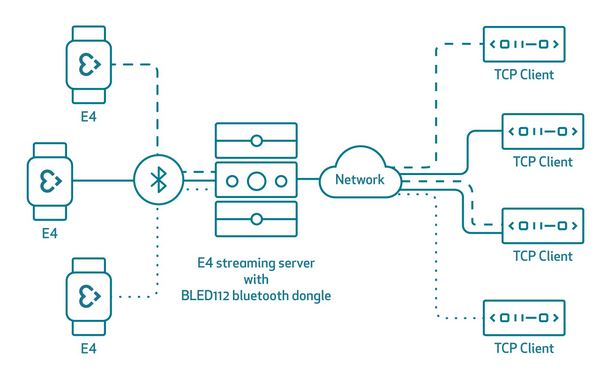
\includegraphics[width=0.75\textwidth]{images/E4streamingServer.JPG}
	\caption[E4 streaming server: connectivity and function]{Illustration of the connectivity and function of the E4 streaming server. On one side are E4s, connected over BTLE to the E4 streaming server using the BLED112 dongle. On the other side are TCP clients, connected to the E4 streaming server through TCP connections over the network. The lines originating from the E4s illustrate the data flow from the E4 through the E4 streaming server to the subscribed TCP client. For example, the data from the first E4 is forwarded by the E4 streaming server to the first and third TCP client. \cite{E4SS}}
	\label{e4ss}
\end{figure}

%Once the TCP clients are connected to the network, as shown in \ref{e4ss}, they are able to communicate with the E4 streaming server. This communication follows a specific message protocol that provides a general structure for client commands and server messages. In general, messages and commands are ASCII strings terminated with a newline character and encoded with UTF-8 \cite{E4MP}. 
\subsection{MATLAB}
MATLAB is a computing and visualization software package, published by MathWorks. It combines a desktop environment tuned for iterative analysis and design processes with a high level programming language for matrix-based mathematics. We used MATLAB (version R2015a) to create a TCP client that was deployed in our data extraction pipeline to send commands to, and receive messages from, the E4 streaming server. Thereby, allowing us to connect an E4 device and control data transmission via a simple user interface.
\subsection{PyCharm}
PyCharm is an integrated development environment (\gls{ide}) for the Python programming language. It is developed by the company JetBrains and provides easy access to a large collection of scientific tools, used for data analysis and visualization. We used PyCharm to manage all data related tasks, such as pre-processing, feature extraction, and machine learning implementation. 

\subsection{PsychoPy}
PsychoPy is an open-source package for running experiments in Python. PsychoPy combines the graphical strengths of OpenGL with the easy Python syntax to give scientists a free and simple stimulus presentation and control package. It is used for psychophysics, cognitive neuroscience and experimental psychology. We used PsychoPy to create and display the paradigm for our experiments. 

\subsection{IAPS}
The International Affective Picture System (IAPS) is being developed to provide a set of normative emotional stimuli for experimental investigations of emotion and attention. The goal of the IAPS is to develop a large set of standardized, emotionally-evocative, internationally-accessible, color photographs that includes contents across a wide range of semantic categories. The IAPS is being developed and distributed by the Center for Emotion and Attention (CSEA) at the University of Florida \cite{Lang2008}.
